\title[HF magnetics I]{High-frequency magnetics I: materials, core loss and the performance factor}
\section{HF magnetics I}

\begin{frame}[plain]
	\titlepage
\end{frame}

%%%%%%%%%%%%%%%%%%%%%%%%%%%%%%%%%%%%%%%%%%%%%%%%%%%%%%%%%%%%%
%% Overview %%
%%%%%%%%%%%%%%%%%%%%%%%%%%%%%%%%%%%%%%%%%%%%%%%%%%%%%%%%%%%%%
\subsection{Flux, loss and size}

\begin{frame}
	\frametitle{Overview}
	In L1 we saw that the magnetic components set the size of a MHz converter. Core loss, not saturation, limits the flux density, and the skin effect limits the useful copper (L7).
	\begin{itemize}
		\item What limits the flux density, and how the VA of a core changes with frequency and size
		\item The loss-optimal flux density
		\item Materials for 1--30\,MHz: MnZn and NiZn ferrites, powders, air core
		\item Core loss for real converter waveforms: iGSE, relaxation, DC bias, data-driven models
		\item Air gaps at high frequency; choosing a material for the design project
	\end{itemize}
	After this lecture you can choose a core material for a MHz converter, set its flux density and estimate its core loss for the actual flux waveform.
\end{frame}

%%%%%%%%%%%%%%%%%%%%%%%%%%%%%%%%%%%%%%%%%%%%%%%%%%%%%%%%%%%%%
%% Recap %%
%%%%%%%%%%%%%%%%%%%%%%%%%%%%%%%%%%%%%%%%%%%%%%%%%%%%%%%%%%%%%
\begin{frame}
	\frametitle{Recap of magnetic basics}
	\begin{columns}[T]
		\begin{column}{0.48\textwidth}
			\small
			\begin{align*}
				v                     & =N A_\mathrm{c}\,\frac{\mathrm{d}B}{\mathrm{d}t}                                   &  & \text{Faraday}       \\
				N i                   & =H_\mathrm{c}l_\mathrm{c}+H_\mathrm{g}l_\mathrm{g}                                   &  & \text{Amp\`ere}      \\
				L                     & =\frac{N^2}{\mathcal{R}_\mathrm{c}+\mathcal{R}_\mathrm{g}},\ \mathcal{R}=\frac{l}{\mu A} &  &                      \\
				P_\mathrm{v}          & =k f^{\alpha}\hat{B}^{\beta}                                                          &  & \text{Steinmetz}     \\
				\delta                & =\sqrt{\rho/(\pi f\mu_0)}                                                             &  & \text{skin depth}
			\end{align*}
		\end{column}
		\begin{column}{0.49\textwidth}
			\small
			From PEDC (L07) and L1:
			\begin{itemize}
				\item Square-wave voltage $V$ on $N$ turns, $D=0.5$: $\hat{B}=V/(4fNA_\mathrm{c})$. At fixed $\hat{B}$ the core could shrink with $1/f$.
				\item $P_\mathrm{v}$ is given for sinusoidal flux; $\hat{B}$ is the amplitude.
				\item Copper at 20\,$^\circ$C: $\delta=66\,\mu$m at 1\,MHz, 21\,$\mu$m at 10\,MHz.
				\item $VA\propto f\hat{B}JA_\mathrm{c}A_\mathrm{w}$; the performance factor $\hat{B}f$ at fixed loss density was measured up to 20\,MHz.
			\end{itemize}
			Today: what limits $\hat{B}$, which material, and how much core loss the real waveform causes.
		\end{column}
	\end{columns}
\end{frame}

%%%%%%%%%%%%%%%%%%%%%%%%%%%%%%%%%%%%%%%%%%%%%%%%%%%%%%%%%%%%%
%% Saturation or loss limit %%
%%%%%%%%%%%%%%%%%%%%%%%%%%%%%%%%%%%%%%%%%%%%%%%%%%%%%%%%%%%%%
\begin{frame}
	\frametitle{Saturation or loss limit}
	\begin{columns}[T]
		\begin{column}{0.48\textwidth}
			\begin{figure}
				\centering
				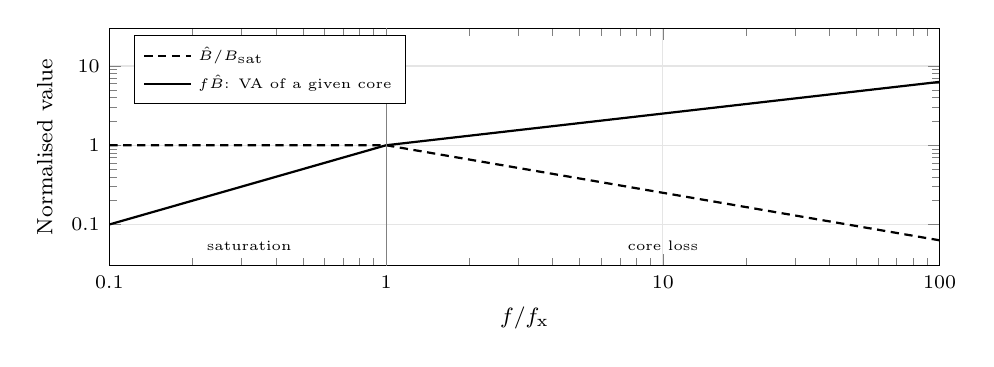
\begin{tikzpicture}
					\begin{loglogaxis}[
							width=\linewidth, height=4.6cm,
							xmin=0.1, xmax=100, ymin=0.03, ymax=30,
							xtick={0.1,1,10,100}, xticklabels={0.1,1,10,100},
							ytick={0.1,1,10}, yticklabels={0.1,1,10},
							xlabel={$f/f_\mathrm{x}$}, ylabel={Normalised value},
							grid=major, grid style={gray!20},
							tick label style={font=\scriptsize}, label style={font=\footnotesize},
							legend style={font=\tiny}, legend pos=north west, legend cell align=left,
						]
						\addplot[black, thick, densely dashed] coordinates {(0.1,1) (1,1) (100,0.0631)};
						\addlegendentry{$\hat{B}/B_\mathrm{sat}$}
						\addplot[black, thick] coordinates {(0.1,0.1) (1,1) (100,6.31)};
						\addlegendentry{$f\hat{B}$: VA of a given core}
						\draw[gray] (axis cs:1,0.03) -- (axis cs:1,30);
						\node[font=\tiny, anchor=south] at (axis cs:0.32,0.035) {saturation};
						\node[font=\tiny, anchor=south] at (axis cs:10,0.035) {core loss};
					\end{loglogaxis}
				\end{tikzpicture}
				\caption{Limit of $\hat{B}$ for $\alpha/\beta=0.6$ (schematic). At $f_\mathrm{x}$ the loss at $B_\mathrm{sat}$ equals the allowed loss density.}
			\end{figure}
		\end{column}
		\begin{column}{0.49\textwidth}
			\small
			At a fixed loss density $P_\mathrm{v}$:
			\begin{equation*}
				\hat{B}=\left(\frac{P_\mathrm{v}}{kf^{\alpha}}\right)^{1/\beta}\quad\Rightarrow\quad f\hat{B}\propto f^{\,1-\alpha/\beta}
			\end{equation*}
			\begin{itemize}
				\item The VA of a given core rises with $f$ only while $\alpha<\beta$.
				\item 3F3 (80\,mW/cm$^3$ at 100\,kHz, 100\,mT, 100\,$^\circ$C; assume $\alpha=1.4$, $\beta=2.5$) reaches 300\,mW/cm$^3$ at 0.3\,T already at about 40\,kHz: every MHz design is loss-limited.
				\item In small or high-$Q$ parts the temperature rise or the efficiency can limit instead (Perreault).
			\end{itemize}
		\end{column}
	\end{columns}
	\blfootnote{Sources: Hanson et al., IEEE TPEL, 2016; Perreault, APEC 2024 plenary; Ferroxcube 3F3 data sheet.}
\end{frame}

%%%%%%%%%%%%%%%%%%%%%%%%%%%%%%%%%%%%%%%%%%%%%%%%%%%%%%%%%%%%%
%% Scaling with size %%
%%%%%%%%%%%%%%%%%%%%%%%%%%%%%%%%%%%%%%%%%%%%%%%%%%%%%%%%%%%%%
\begin{frame}
	\frametitle{Small magnetics are inefficient}
	\begin{columns}[T]
		\begin{column}{0.52\textwidth}
			\begin{table}
				\centering
				\footnotesize
				\begin{tabular}{|l|l|l|}
					\hline
					\textbf{Fixed quantity}         & \textbf{VA}                    & \textbf{VA/volume}               \\
					\hline
					\multicolumn{3}{|l|}{\textit{windings without skin effect}}                                       \\
					loss density                    & $\varepsilon^{4}$              & $\varepsilon$                    \\
					heat flux per surface           & $\varepsilon^{3.1}$            & $\varepsilon^{0.1}$              \\
					efficiency                      & $\varepsilon^{13}$             & $\varepsilon^{10}$               \\
					\hline
					\multicolumn{3}{|l|}{\textit{HF windings (skin effect)}}                                          \\
					heat flux per surface           & $\varepsilon^{2.6}$            & $\varepsilon^{-0.4}$             \\
					efficiency                      & $\varepsilon^{8}$              & $\varepsilon^{5}$                \\
					\hline
				\end{tabular}
				\caption{Scaling of a magnetic component with its linear dimension $\varepsilon$ (Steinmetz $\beta=2.5$)}
			\end{table}
		\end{column}
		\begin{column}{0.45\textwidth}
			\small
			\begin{itemize}
				\item At constant loss density the loss fraction grows as $1/\varepsilon$: small parts become inefficient before they become hot.
				\item Small components are therefore limited by efficiency. At fixed efficiency, halving all dimensions of an HF inductor divides its VA by $2^8=256$.
				\item Magnetics cannot be built from many small cells, as capacitors and transistors can.
			\end{itemize}
			\begin{block}{Key message}
				Use few, large magnetic components and fill the available volume.
			\end{block}
		\end{column}
	\end{columns}
	\blfootnote{Source: Sullivan, Reese, Stein, Kyaw, 3D-PEIM 2016, Tab.\ I.}
\end{frame}

%%%%%%%%%%%%%%%%%%%%%%%%%%%%%%%%%%%%%%%%%%%%%%%%%%%%%%%%%%%%%
%% Modified performance factor %%
%%%%%%%%%%%%%%%%%%%%%%%%%%%%%%%%%%%%%%%%%%%%%%%%%%%%%%%%%%%%%
\begin{frame}
	\frametitle{Winding loss and frequency}
	\begin{columns}[T]
		\begin{column}{0.46\textwidth}
			\begin{figure}
				\centering
				\begin{tikzpicture}
					\begin{semilogxaxis}[
							width=\linewidth, height=4.6cm,
							xmin=1.8, xmax=22, ymin=0.5, ymax=2.5,
							xtick={2,5,10,20}, xticklabels={2,5,10,20},
							xlabel={Frequency (MHz)}, ylabel={$F_w/F_w(2\,\mathrm{MHz})$},
							grid=major, grid style={gray!20},
							tick label style={font=\scriptsize}, label style={font=\footnotesize},
							legend style={font=\tiny}, legend pos=north west, legend cell align=left,
						]
						\addplot[black, thick, mark=*, mark size=1.3pt] table[x=f_MHz, y=F1] {fig/lec06/fw_norm_fr67.dat};
						\addlegendentry{$\hat{B}f$}
						\addplot[black, thick, dashed, mark=square*, mark size=1.3pt] table[x=f_MHz, y=F34] {fig/lec06/fw_norm_fr67.dat};
						\addlegendentry{$\hat{B}f^{3/4}$}
						\addplot[gray, thick, mark=triangle*, mark size=1.6pt] table[x=f_MHz, y=F12] {fig/lec06/fw_norm_fr67.dat};
						\addlegendentry{$\hat{B}f^{1/2}$}
					\end{semilogxaxis}
				\end{tikzpicture}
				\caption{Fair-Rite 67 at 500\,mW/cm$^3$, data of Hanson et al.\ (2016)}
			\end{figure}
		\end{column}
		\begin{column}{0.51\textwidth}
			\small
			At fixed winding loss $I\propto R_\mathrm{ac}^{-1/2}$, and $VA\propto N\hat{B}f\cdot I/N$:
			\begin{table}
				\centering
				\footnotesize
				\begin{tabular}{|>{\raggedright\arraybackslash}p{3.6cm}|l|l|}
					\hline
					\textbf{Winding}                                        & $R_\mathrm{ac}\propto$ & \textbf{Metric}  \\
					\hline
					no skin or proximity effect                             & $f^0$                  & $\hat{B}f$       \\
					single layer, or fixed number of layers with optimal thickness & $f^{1/2}$       & $\hat{B}f^{3/4}$ \\
					fixed layer or strand thickness (litz, 32\,$\mu$m)      & $f$                    & $\hat{B}f^{1/2}$ \\
					\hline
				\end{tabular}
			\end{table}
			From 2 to 10\,MHz: $\hat{B}f$ $\times2.1$, $\hat{B}f^{3/4}$ $\times1.4$, $\hat{B}f^{1/2}$ $\times0.95$. With single-layer windings the power density rises by 40--45\,\%; litz wire gives no benefit. L7 designs the winding.
		\end{column}
	\end{columns}
	\blfootnote{Source: Hanson et al., IEEE TPEL, vol.\ 31, no.\ 11, 2016, Tab.\ I and II.}
\end{frame}

%%%%%%%%%%%%%%%%%%%%%%%%%%%%%%%%%%%%%%%%%%%%%%%%%%%%%%%%%%%%%
%% Task: two materials %%
%%%%%%%%%%%%%%%%%%%%%%%%%%%%%%%%%%%%%%%%%%%%%%%%%%%%%%%%%%%%%
% Two pages: task (page 1) and task with solution (page 2).
\begin{frame}<handout:1-2>
	\frametitle{Comparing two materials}
	\begin{block}{Task (4 minutes)}
		Steinmetz fits at 10\,MHz by Hanson et al.\ ($P_\mathrm{v}=k\hat{B}^{\beta}$, $P_\mathrm{v}$ in mW/cm$^3$, $\hat{B}$ in mT): Fair-Rite 67 ($\mu_\mathrm{r}=40$): $k=2.09$, $\beta=2.08$. Ferroxcube 4F1 ($\mu_\mathrm{r}=80$): $k=2.86$, $\beta=2.28$.
		\begin{enumerate}
			\item Calculate $\hat{B}$ and $\hat{B}f$ of both materials for $P_\mathrm{v}=500$\,mW/cm$^3$.
			\item Repeat for 200\,mW/cm$^3$ (natural convection).
			\item Which material lets a given core handle more VA, and by how much?
		\end{enumerate}
	\end{block}
	\onslide<2-|handout:2>{
		\begin{enumerate}
			\item 67: $\hat{B}=(500/2.09)^{1/2.08}=13.9$\,mT, $\hat{B}f=139$\,mT$\cdot$MHz. 4F1: $(500/2.86)^{1/2.28}=9.6$\,mT, 96\,mT$\cdot$MHz.
			\item 67: 9.0\,mT, 4F1: 6.4\,mT.
			\item Same core and winding, $VA\propto\hat{B}f$: 67 handles 1.45 times the VA (1.39 times at 200\,mW/cm$^3$). Its lower permeability is no drawback: the inductor needs a gap anyway.
		\end{enumerate}
	}
\end{frame}

%%%%%%%%%%%%%%%%%%%%%%%%%%%%%%%%%%%%%%%%%%%%%%%%%%%%%%%%%%%%%
%% Optimum flux density %%
%%%%%%%%%%%%%%%%%%%%%%%%%%%%%%%%%%%%%%%%%%%%%%%%%%%%%%%%%%%%%
\begin{frame}
	\frametitle{Optimum flux density}
	\begin{columns}[T]
		\begin{column}{0.46\textwidth}
			\begin{figure}
				\centering
				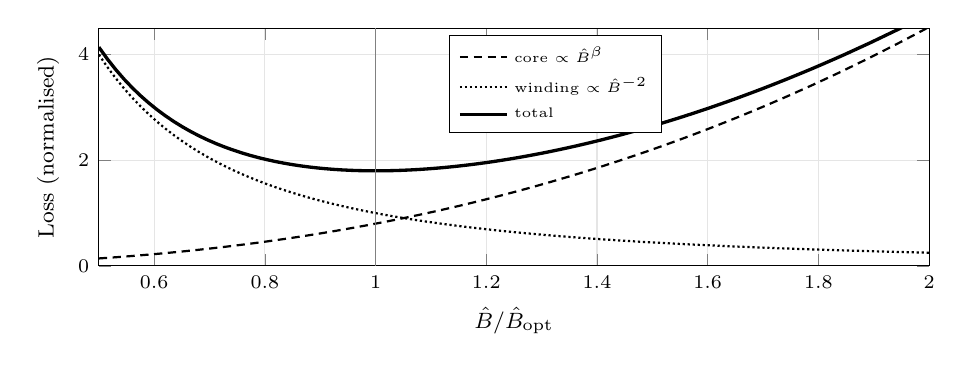
\begin{tikzpicture}
					\begin{axis}[
							width=\linewidth, height=4.6cm,
							xmin=0.5, xmax=2, ymin=0, ymax=4.5,
							xlabel={$\hat{B}/\hat{B}_\mathrm{opt}$}, ylabel={Loss (normalised)},
							grid=major, grid style={gray!20},
							tick label style={font=\scriptsize}, label style={font=\footnotesize},
							legend style={font=\tiny, at={(0.55,0.97)}, anchor=north}, legend cell align=left,
						]
						\addplot[black, thick, densely dashed, domain=0.5:2, samples=100] {0.8*x^2.5};
						\addlegendentry{core $\propto\hat{B}^{\beta}$}
						\addplot[black, thick, densely dotted, domain=0.5:2, samples=100] {1/x^2};
						\addlegendentry{winding $\propto\hat{B}^{-2}$}
						\addplot[black, very thick, domain=0.5:2, samples=100] {0.8*x^2.5+1/x^2};
						\addlegendentry{total}
						\draw[gray] (axis cs:1,0) -- (axis cs:1,4.5);
					\end{axis}
				\end{tikzpicture}
				\caption{Core, winding and total loss for $\beta=2.5$}
			\end{figure}
		\end{column}
		\begin{column}{0.51\textwidth}
			\small
			For a given volt-second product $N\propto1/\hat{B}$. With the window always filled $P_\mathrm{cu}\propto N^2\propto\hat{B}^{-2}$, while $P_\mathrm{fe}\propto\hat{B}^{\beta}$:
			\begin{equation*}
				\frac{\mathrm{d}P_\mathrm{tot}}{\mathrm{d}\hat{B}}=0\quad\Rightarrow\quad P_\mathrm{fe}=\frac{2}{\beta}\,P_\mathrm{cu}
			\end{equation*}
			\begin{itemize}
				\item Not at equal losses: $\beta=2.5$ gives $P_\mathrm{fe}=0.8\,P_\mathrm{cu}$; at HF ($\beta\approx2$) nearly equal.
				\item Flat minimum: 20\,\% below or 25\,\% above $\hat{B}_\mathrm{opt}$ costs 12--13\,\% more loss.
				\item $R\propto N^2$ also holds for a single-layer winding with skin effect and fixed breadth.
			\end{itemize}
		\end{column}
	\end{columns}
	\blfootnote{Source: Erickson and Maksimovi\'c, \textit{Fundamentals of Power Electronics}, 3rd ed., 2020, Sec.\ 12.1.5.}
\end{frame}

%%%%%%%%%%%%%%%%%%%%%%%%%%%%%%%%%%%%%%%%%%%%%%%%%%%%%%%%%%%%%
%% Task: optimum flux density %%
%%%%%%%%%%%%%%%%%%%%%%%%%%%%%%%%%%%%%%%%%%%%%%%%%%%%%%%%%%%%%
% Two pages: task (page 1) and task with solution (page 2).
\begin{frame}<handout:1-2>
	\frametitle{Finding the optimum}
	\begin{block}{Task (4 minutes)}
		An inductor at 5\,MHz has $N=6$ turns and runs at $\hat{B}=20$\,mT. Core loss 1.2\,W, winding loss 0.4\,W, $\beta=2.2$. The winding fills the window for every $N$.
		\begin{enumerate}
			\item Which $\hat{B}$ gives the lowest total loss, and how large are the losses?
			\item How many turns does this need?
			\item How much is lost with one turn less?
		\end{enumerate}
	\end{block}
	\onslide<2-|handout:2>{
		\begin{enumerate}
			\item With $x=\hat{B}/20\,\mathrm{mT}$: $\beta\cdot1.2\,x^{\beta}=2\cdot0.4\,x^{-2}$ $\Rightarrow$ $x^{4.2}=0.303$, $x=0.753$, $\hat{B}=15.1$\,mT. $P_\mathrm{fe}=0.64$\,W, $P_\mathrm{cu}=0.71$\,W, total 1.35\,W instead of 1.60\,W ($-16$\,\%).
			\item $N\propto1/\hat{B}$: $N=6/0.753=8.0$, i.e.\ 8 turns.
			\item 7 turns: $\hat{B}=17.1$\,mT, 1.40\,W, only 4\,\% more. Fewer turns also mean less winding capacitance (L7).
		\end{enumerate}
	}
\end{frame}

%%%%%%%%%%%%%%%%%%%%%%%%%%%%%%%%%%%%%%%%%%%%%%%%%%%%%%%%%%%%%
%% Material families %%
%%%%%%%%%%%%%%%%%%%%%%%%%%%%%%%%%%%%%%%%%%%%%%%%%%%%%%%%%%%%%
\subsection{Materials for MHz}

\begin{frame}
	\frametitle{Material families}
	\begin{table}
		\centering
		\footnotesize
		\begin{tabular}{|>{\raggedright\arraybackslash}p{3.3cm}|l|>{\raggedright\arraybackslash}p{2.0cm}|>{\raggedright\arraybackslash}p{2.1cm}|>{\raggedright\arraybackslash}p{4.6cm}|}
			\hline
			\textbf{Material}                                & $\mu_\mathrm{i}$ & \textbf{Resistivity}        & \textbf{Range}            & \textbf{Remarks}                                                         \\
			\hline
			MnZn ferrite (3F3, 3F4, 3F46)                    & 750--2000        & 2--10\,$\Omega$m            & up to about 3\,MHz        & high $\mu$ and permittivity: eddy currents and dimensional resonance in large cores \\
			NiZn ferrite (4F1, Fair-Rite 61, 67)             & 40--125          & $\approx10^5\,\Omega$m      & 2--50\,MHz                & highest performance factor in the HF range, often at $\mu_\mathrm{r}=20$--40 \\
			carbonyl-iron powder (Micrometals -2, -17)       & 4--10            & insulated particles         & data at 10--70\,MHz       & distributed gap; at 10\,MHz $\hat{B}f=62$ vs.\ 139\,mT$\cdot$MHz of 67 \\
			nanocrystalline and amorphous tape               & very high        & thin metal tape             & up to some 100\,kHz       & $B_\mathrm{sat}=1.2$--1.6\,T; chokes, EMI filters, LF transformers \\
			thin films (e.g.\ NiFe, CoZrTa, Co-Zr-O)          & high             & laminated or granular       & 5--100\,MHz               & inductors on chip and in the package (L7)                               \\
			air core                                         & 1                & --                          & any                       & no core loss and no saturation; stray field and size                    \\
			\hline
		\end{tabular}
		\caption{Magnetic materials for power conversion (manufacturer data; Hanson et al., 2016)}
	\end{table}
	\blfootnote{Sources: Ferroxcube and Fair-Rite data sheets; Hanson et al., 2016; \'O Math\'una et al., 2012.}
\end{frame}

%%%%%%%%%%%%%%%%%%%%%%%%%%%%%%%%%%%%%%%%%%%%%%%%%%%%%%%%%%%%%
%% Poll: MnZn or NiZn %%
%%%%%%%%%%%%%%%%%%%%%%%%%%%%%%%%%%%%%%%%%%%%%%%%%%%%%%%%%%%%%
% Two pages: question (page 1) and answer (page 2).
\begin{frame}<handout:1-2>
	\frametitle{MnZn or NiZn at 10\,MHz?}
	A resonant inductor for 10\,MHz needs a core. Vote, then discuss with your neighbour (2 minutes).
	\begin{enumerate}[(a)]
		\item MnZn ferrite 3F4 ($\mu_\mathrm{i}=900$): more inductance per turn
		\item NiZn ferrite 4F1 ($\mu_\mathrm{i}=80$): less core loss at 10\,MHz
		\item it does not matter, with a gap both behave the same
		\item no core at all
	\end{enumerate}
	\onslide<2-|handout:2>{
		\begin{block}{Answer: (b), and (d) is worth checking}
			MnZn has about $10^4$ times lower resistivity, so eddy currents flow in the core. Its high permeability brings the drop of $\mu'$ and the rise of $\mu''$ down to a few MHz (next slide). Its high permittivity ($\varepsilon_\mathrm{r}\approx10^4$ and more) shortens the wavelength in the core to centimetres: larger cores show standing waves (dimensional resonance). The high $\mu$ is lost in the gap anyway. 3F4 is specified for 1--2\,MHz, 4F1 for 4--10\,MHz. A gap changes the inductance, not the loss density at a given $\hat{B}$. An air core can win at higher frequency or for very high $Q$.
		\end{block}
	}
	\blfootnote{Sources: Ferroxcube data sheets; Skutt, PhD thesis, Virginia Tech, 1996; Hanson et al., 2016.}
\end{frame}

%%%%%%%%%%%%%%%%%%%%%%%%%%%%%%%%%%%%%%%%%%%%%%%%%%%%%%%%%%%%%
%% Complex permeability %%
%%%%%%%%%%%%%%%%%%%%%%%%%%%%%%%%%%%%%%%%%%%%%%%%%%%%%%%%%%%%%
\begin{frame}
	\frametitle{Complex permeability}
	\begin{columns}[T]
		\begin{column}{0.48\textwidth}
			\begin{figure}
				\centering
				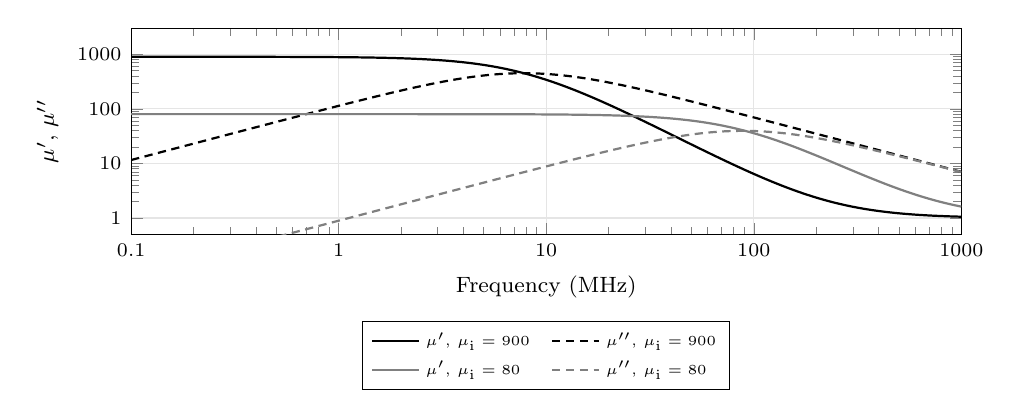
\begin{tikzpicture}
					\begin{loglogaxis}[
							width=\linewidth, height=4.2cm,
							xmin=0.1, xmax=1000, ymin=0.5, ymax=3000,
							xtick={0.1,1,10,100,1000}, xticklabels={0.1,1,10,100,1000},
							ytick={1,10,100,1000}, yticklabels={1,10,100,1000},
							xlabel={Frequency (MHz)}, ylabel={$\mu'$, $\mu''$},
							grid=major, grid style={gray!20},
							tick label style={font=\scriptsize}, label style={font=\footnotesize},
							legend style={font=\tiny, at={(0.5,-0.42)}, anchor=north, legend columns=2, /tikz/every even column/.append style={column sep=0.2cm}}, legend cell align=left,
						]
						% relaxation model mu = 1 + (mu_i-1)/(1 + j f/f_r), Snoek product 7 GHz
						\addplot[black, thick, domain=-1:3, samples=200] ({10^x}, {1+899/(1+(10^x/7.79)^2)});
						\addlegendentry{$\mu'$, $\mu_\mathrm{i}=900$}
						\addplot[black, thick, densely dashed, domain=-1:3, samples=200] ({10^x}, {899*(10^x/7.79)/(1+(10^x/7.79)^2)});
						\addlegendentry{$\mu''$, $\mu_\mathrm{i}=900$}
						\addplot[gray, thick, domain=-1:3, samples=200] ({10^x}, {1+79/(1+(10^x/88.6)^2)});
						\addlegendentry{$\mu'$, $\mu_\mathrm{i}=80$}
						\addplot[gray, thick, densely dashed, domain=-1:3, samples=200] ({10^x}, {79*(10^x/88.6)/(1+(10^x/88.6)^2)});
						\addlegendentry{$\mu''$, $\mu_\mathrm{i}=80$}
					\end{loglogaxis}
				\end{tikzpicture}
				\caption{Relaxation model $\mu=1+(\mu_\mathrm{i}-1)/(1+\mathrm{j}f/f_\mathrm{r})$, Snoek's product 7\,GHz (schematic)}
			\end{figure}
		\end{column}
		\begin{column}{0.49\textwidth}
			\small
			\begin{itemize}
				\item $\mu=\mu'-\mathrm{j}\mu''$: $\mu'$ stores energy, $\mu''$ dissipates it. Small-signal $Q$ of the core: $\mu'/\mu''$.
				\item Snoek's law for spinel ferrites:
				      \begin{equation*}
					      (\mu_\mathrm{i}-1)\,f_\mathrm{r}\approx\frac{2}{3}\,\frac{\gamma}{2\pi}\,\mu_0M_\mathrm{s}\approx5\text{--}9\,\mathrm{GHz}
				      \end{equation*}
				      with $\gamma/2\pi=28$\,GHz/T and $\mu_0M_\mathrm{s}=0.3$--0.5\,T.
				\item $\mu_\mathrm{i}=2000$: $f_\mathrm{r}\approx3$--5\,MHz; $\mu_\mathrm{i}=80$: 70--120\,MHz. High permeability and high frequency exclude each other.
				\item Small-signal data ($\mu''$) do not predict the loss at power-level flux: measure at the operating $\hat{B}$.
			\end{itemize}
		\end{column}
	\end{columns}
	\blfootnote{Sources: J.\,L. Snoek, Physica, vol.\ 14, 1948; Hanson et al., 2016, Sec.\ III.}
\end{frame}

%%%%%%%%%%%%%%%%%%%%%%%%%%%%%%%%%%%%%%%%%%%%%%%%%%%%%%%%%%%%%
%% How much permeability %%
%%%%%%%%%%%%%%%%%%%%%%%%%%%%%%%%%%%%%%%%%%%%%%%%%%%%%%%%%%%%%
\begin{frame}
	\frametitle{How much permeability?}
	\begin{columns}[T]
		\begin{column}{0.42\textwidth}
			\begin{figure}
				\centering
				\begin{circuitikz}[scale=0.85, transform shape]
					\draw (0,0) to[V, v=$Ni$] (0,2.4) to[R, l=$\mathcal{R}_\mathrm{c}$, i=$\Phi$] (3.2,2.4) to[R, l=$\mathcal{R}_\mathrm{g}$] (3.2,0) -- (0,0);
				\end{circuitikz}
				\caption{Magnetic circuit of a gapped core}
			\end{figure}
			\small
			\begin{equation*}
				L=\frac{\mu_0N^2A_\mathrm{c}}{l_\mathrm{g}+l_\mathrm{c}/\mu_\mathrm{r}}
			\end{equation*}
			(gap area taken equal to $A_\mathrm{c}$)
		\end{column}
		\begin{column}{0.55\textwidth}
			\small
			Without gap, $N$ turns give the required $L$ only with
			\begin{equation*}
				\mu_\mathrm{r,th}=\frac{L\,l_\mathrm{c}}{\mu_0N^2A_\mathrm{c}}
			\end{equation*}
			\begin{itemize}
				\item $\mu_\mathrm{r}>\mu_\mathrm{r,th}$: a gap is needed, and more permeability only changes the gap length.
				\item $\mu_\mathrm{r}<\mu_\mathrm{r,th}$: more turns are needed, and the winding loss rises.
				\item Example: 1\,$\mu$H with $N=10$, $l_\mathrm{c}=30$\,mm, $A_\mathrm{c}=20$\,mm$^2$: $\mu_\mathrm{r,th}=12$. A material with $\mu_\mathrm{r}=40$ already needs a gap.
				\item The best HF materials have $\mu_\mathrm{r}\approx20$--40.
			\end{itemize}
		\end{column}
	\end{columns}
	\blfootnote{Source: Hanson et al., IEEE TPEL, 2016, Sec.\ V.}
\end{frame}

%%%%%%%%%%%%%%%%%%%%%%%%%%%%%%%%%%%%%%%%%%%%%%%%%%%%%%%%%%%%%
%% Temperature %%
%%%%%%%%%%%%%%%%%%%%%%%%%%%%%%%%%%%%%%%%%%%%%%%%%%%%%%%%%%%%%
\begin{frame}
	\frametitle{Temperature dependence}
	\begin{columns}[T]
		\begin{column}{0.52\textwidth}
			\small
			\begin{itemize}
				\item MnZn power ferrites are doped so that the loss minimum lies at 80--100\,$^\circ$C, the usual operating temperature. Above the minimum the loss rises with temperature: with weak cooling the core can run away thermally.
				\item Above about 1\,MHz the temperature dependence of the loss of MnZn ferrites flattens.
				\item The flux density at a given field falls with temperature.
				\item Data sheets give typical ($\approx$) or maximum ($\leq$) values, mostly at 100\,$^\circ$C. Core loss differs between lots by 20\,\% or more: keep a margin.
			\end{itemize}
		\end{column}
		\begin{column}{0.45\textwidth}
			\begin{table}
				\centering
				\footnotesize
				\begin{tabular}{|l|l|l|l|}
					\hline
					\textbf{Material} & \multicolumn{2}{l|}{\textbf{$B$ in mT}} & $T_\mathrm{C}$ in $^\circ$C \\
					                  & 25\,$^\circ$C & 100\,$^\circ$C          &                               \\
					\hline
					3F3               & 440           & 370                     & $\geq200$                     \\
					3F4               & 410           & 350                     & $\geq220$                     \\
					3F46              & 520           & 430                     & $\geq280$                     \\
					4F1               & 320           & 260                     & $\geq260$                     \\
					Fair-Rite 67      & 230           & --                      & $>450$                        \\
					\hline
				\end{tabular}
				\caption{Flux density at 1200\,A/m (MnZn), 3000\,A/m (4F1) and 1600\,A/m (67); Curie temperature}
			\end{table}
		\end{column}
	\end{columns}
	\blfootnote{Sources: Beatrice et al., J.\ Appl.\ Phys., 2019; Ferroxcube and Fair-Rite data sheets; Hanson et al., 2016.}
\end{frame}

%%%%%%%%%%%%%%%%%%%%%%%%%%%%%%%%%%%%%%%%%%%%%%%%%%%%%%%%%%%%%
%% Steinmetz limits %%
%%%%%%%%%%%%%%%%%%%%%%%%%%%%%%%%%%%%%%%%%%%%%%%%%%%%%%%%%%%%%
\subsection{Core-loss models}

\begin{frame}
	\frametitle{Steinmetz and its limits}
	\begin{columns}[T]
		\begin{column}{0.46\textwidth}
			\begin{figure}
				\centering
				\begin{tikzpicture}
					\begin{loglogaxis}[
							width=\linewidth, height=4.6cm,
							xmin=1.8, xmax=22, ymin=20, ymax=1500,
							xtick={2,5,10,20}, xticklabels={2,5,10,20},
							ytick={30,100,300,1000}, yticklabels={30,100,300,1000},
							xlabel={Frequency (MHz)}, ylabel={$P_\mathrm{v}$ (mW/cm$^3$)},
							grid=major, grid style={gray!20},
							tick label style={font=\scriptsize}, label style={font=\footnotesize},
						]
						\addplot[black, only marks, mark=*, mark size=1.5pt] table[x=f_MHz, y=Pv] {fig/lec06/pv_fr67_10mT.dat};
						\addplot[gray, domain=2:10, samples=2] {27.5*(x/2)^1.4};
						\addplot[gray, densely dashed, domain=10:20, samples=2] {251.3*(x/10)^2.1};
						\node[font=\tiny, anchor=south east] at (axis cs:4.5,80) {$\propto f^{1.4}$};
						\node[font=\tiny, anchor=north west] at (axis cs:13,380) {$\propto f^{2.1}$};
					\end{loglogaxis}
				\end{tikzpicture}
				\caption{Fair-Rite 67 at $\hat{B}=10$\,mT (data of Hanson et al., 2016)}
			\end{figure}
		\end{column}
		\begin{column}{0.51\textwidth}
			\small
			\begin{itemize}
				\item $P_\mathrm{v}=kf^{\alpha}\hat{B}^{\beta}$ is a fit to sinusoidal data at one temperature, without DC bias, over a limited range of $f$ and $\hat{B}$.
				\item At HF the parameters change with frequency. Fair-Rite 67: $\beta=2.44$ at 2\,MHz, 1.99 at 20\,MHz; $\alpha\approx1.4$ below and 2.1 above 10\,MHz. Where $\alpha>\beta$, $\hat{B}f$ falls.
				\item Converter flux is rarely sinusoidal: triangular (buck, boost, TCM), trapezoidal with zero-voltage intervals (three-level bridge voltage), with DC bias (inductors).
				\item Adding the losses of the harmonics is wrong: core loss is not linear in $B$.
			\end{itemize}
		\end{column}
	\end{columns}
	\blfootnote{Source: Hanson et al., IEEE TPEL, 2016, Tab.\ II and App.\ C.}
\end{frame}

%%%%%%%%%%%%%%%%%%%%%%%%%%%%%%%%%%%%%%%%%%%%%%%%%%%%%%%%%%%%%
%% iGSE %%
%%%%%%%%%%%%%%%%%%%%%%%%%%%%%%%%%%%%%%%%%%%%%%%%%%%%%%%%%%%%%
\begin{frame}
	\frametitle{Loss with non-sinusoidal flux}
	\begin{columns}[T]
		\begin{column}{0.46\textwidth}
			\begin{figure}
				\centering
				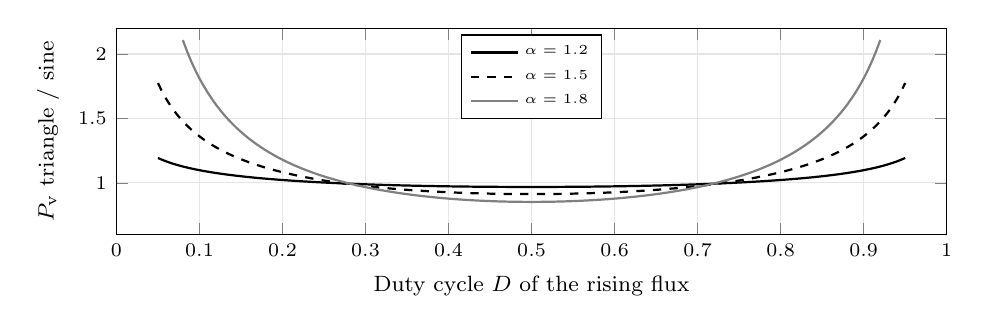
\begin{tikzpicture}
					\begin{axis}[
							width=\linewidth, height=4.2cm,
							xmin=0, xmax=1, ymin=0.6, ymax=2.2,
							xlabel={Duty cycle $D$ of the rising flux}, ylabel={$P_\mathrm{v}$ triangle / sine},
							grid=major, grid style={gray!20},
							tick label style={font=\scriptsize}, label style={font=\footnotesize},
							legend style={font=\tiny, at={(0.5,0.97)}, anchor=north}, legend cell align=left,
						]
						% iGSE: ratio = C_alpha (D^(1-alpha) + (1-D)^(1-alpha)), C_alpha = 2^alpha/((2 pi)^(alpha-1) int |cos|^alpha)
						\addplot[black, thick, domain=0.05:0.95, samples=181] {0.42146*(x^(-0.2)+(1-x)^(-0.2))};
						\addlegendentry{$\alpha=1.2$}
						\addplot[black, thick, dashed, domain=0.05:0.95, samples=181] {0.32276*(x^(-0.5)+(1-x)^(-0.5))};
						\addlegendentry{$\alpha=1.5$}
						\addplot[gray, thick, domain=0.08:0.92, samples=169] {0.24475*(x^(-0.8)+(1-x)^(-0.8))};
						\addlegendentry{$\alpha=1.8$}
					\end{axis}
				\end{tikzpicture}
				\caption{Triangular flux with the same $\hat{B}$ and $f$ as the sine}
			\end{figure}
			\small
			Triangle, $\Delta B=2\hat{B}$ peak to peak:
			\begin{equation*}
				P_\mathrm{v}=k_\mathrm{i}(\Delta B)^{\beta}f^{\alpha}\left(D^{1-\alpha}+(1-D)^{1-\alpha}\right)
			\end{equation*}
		\end{column}
		\begin{column}{0.51\textwidth}
			\small
			Improved generalised Steinmetz equation (iGSE):
			\begin{equation*}
				P_\mathrm{v}=\frac{1}{T}\int_0^Tk_\mathrm{i}\left|\frac{\mathrm{d}B}{\mathrm{d}t}\right|^{\alpha}(\Delta B)^{\beta-\alpha}\,\mathrm{d}t
			\end{equation*}
			\begin{equation*}
				k_\mathrm{i}=\frac{k}{(2\pi)^{\alpha-1}\int_0^{2\pi}|\cos\theta|^{\alpha}\,2^{\beta-\alpha}\,\mathrm{d}\theta}
			\end{equation*}
			\begin{itemize}
				\item $\Delta B$: peak-to-peak value of the major loop; minor loops are treated separately.
				\item Only $k$, $\alpha$, $\beta$ of the sine data are needed.
				\item Fast flux edges cost more: $D=0.1$ and $\alpha=1.5$ give 36\,\% more than the sine.
			\end{itemize}
		\end{column}
	\end{columns}
	\blfootnote{Source: Venkatachalam, Sullivan, Abdallah, Tacca, IEEE COMPEL 2002, pp.\ 36--41.}
\end{frame}

%%%%%%%%%%%%%%%%%%%%%%%%%%%%%%%%%%%%%%%%%%%%%%%%%%%%%%%%%%%%%
%% Relaxation and DC bias %%
%%%%%%%%%%%%%%%%%%%%%%%%%%%%%%%%%%%%%%%%%%%%%%%%%%%%%%%%%%%%%
\begin{frame}
	\frametitle{Relaxation and DC bias}
	\begin{columns}[T]
		\begin{column}{0.42\textwidth}
			\begin{figure}
				\centering
				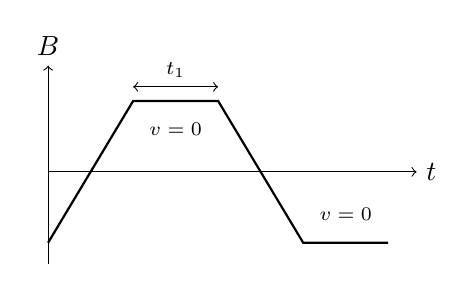
\begin{tikzpicture}[scale=0.9]
					\draw[->] (0,0) -- (5.2,0) node[right]{$t$};
					\draw[->] (0,-1.3) -- (0,1.5) node[above]{$B$};
					\draw[thick] (0,-1) -- (1.2,1) -- (2.4,1) -- (3.6,-1) -- (4.8,-1);
					\draw[<->] (1.2,1.2) -- (2.4,1.2) node[midway, above, font=\scriptsize]{$t_1$};
					\node[font=\scriptsize] at (1.8,0.6) {$v=0$};
					\node[font=\scriptsize] at (4.2,-0.6) {$v=0$};
				\end{tikzpicture}
				\caption{Flux with zero-voltage intervals (three-level bridge voltage)}
			\end{figure}
		\end{column}
		\begin{column}{0.55\textwidth}
			\small
			\begin{itemize}
				\item While $v=0$ the iGSE predicts no loss. Measurements show extra loss after each step to zero voltage: relaxation. The i$^2$GSE adds a term that grows with $1-\mathrm{e}^{-t_1/\tau}$ (N87: $\tau=6\,\mu$s). It matters for three-level bridge voltages and for DCM.
				\item A DC flux raises the loss, even far below saturation. NiZn ferrite ($\mu_\mathrm{r}=125$) at 10\,MHz and 6.5\,mT ac: at least three times the loss, with hysteresis. Heuristic: DC flux not larger than the allowed ac amplitude.
				\item The permeability changes with the bias, and so does $L$.
				\item Model with the iGSE, then check with the real waveform (L5: resonant or calorimetric method).
			\end{itemize}
		\end{column}
	\end{columns}
	\blfootnote{Sources: M\"uhlethaler, Biela, Kolar, Ecklebe, IEEE TPEL, vol.\ 27, no.\ 2, 2012; Hanson et al., 2016, App.\ C.}
\end{frame}

%%%%%%%%%%%%%%%%%%%%%%%%%%%%%%%%%%%%%%%%%%%%%%%%%%%%%%%%%%%%%
%% Data-driven models %%
%%%%%%%%%%%%%%%%%%%%%%%%%%%%%%%%%%%%%%%%%%%%%%%%%%%%%%%%%%%%%
\begin{frame}
	\frametitle{Data-driven core-loss models}
	\begin{columns}[T]
		\begin{column}{0.5\textwidth}
			\small
			\textbf{MagNet database}
			\begin{itemize}
				\item Open data of measured $B$--$H$ loops: 10 ferrites (e.g.\ N87), more than 500\,000 waveforms (sine, triangle, trapezoid).
				\item 50--500\,kHz, 25--90\,$^\circ$C, with DC bias; automated two-winding set-up in an oil bath.
				\item The MagNet Challenge 2023 was an open competition for compact and accurate models.
			\end{itemize}
		\end{column}
		\begin{column}{0.47\textwidth}
			\small
			\textbf{Neural networks as data sheets}
			\begin{itemize}
				\item Inputs: $B(t)$, $f$, temperature, DC bias. Outputs: $P_\mathrm{v}$ or the whole $H(t)$ and thus the loop.
				\item Transfer learning: about 100 measured points adapt a trained model to a new material.
			\end{itemize}
			\begin{block}{In the MHz range}
				No comparable open data exist yet. Use published fits (Hanson et al.), data sheets and your own resonant measurements (L5, Tutorial 6).
			\end{block}
		\end{column}
	\end{columns}
	\blfootnote{Sources: Li et al., IEEE TPEL, vol.\ 38, no.\ 12, 2023; Chen et al., IEEE Open J.\ Power Electron., vol.\ 6, 2025.}
\end{frame}

%%%%%%%%%%%%%%%%%%%%%%%%%%%%%%%%%%%%%%%%%%%%%%%%%%%%%%%%%%%%%
%% Reading a datasheet %%
%%%%%%%%%%%%%%%%%%%%%%%%%%%%%%%%%%%%%%%%%%%%%%%%%%%%%%%%%%%%%
\begin{frame}
	\frametitle{Reading a core-loss datasheet}
	\begin{columns}[T]
		\begin{column}{0.5\textwidth}
			\small
			\begin{itemize}
				\item Units: 1\,mW/cm$^3$ = 1\,kW/m$^3$.
				\item $\hat{B}$ is the amplitude. Using the peak-to-peak value instead multiplies the loss by $2^{\beta}$, i.e.\ 4 to 8.
				\item Conditions: sinusoidal flux, small toroid, often 100\,$^\circ$C; typical or maximum values.
				\item $\beta$ from two points at one frequency:
				      \begin{equation*}
					      \beta=\frac{\ln(P_2/P_1)}{\ln(\hat{B}_2/\hat{B}_1)}
				      \end{equation*}
				\item Core loss $=P_\mathrm{v}V_\mathrm{e}$, with the effective volume $V_\mathrm{e}$ of the core data sheet.
			\end{itemize}
		\end{column}
		\begin{column}{0.47\textwidth}
			\small
			\textbf{Example: 3F46 at 3\,MHz, 100\,$^\circ$C}
			\begin{itemize}
				\item 10\,mT: $\approx50$\,kW/m$^3$; 30\,mT: $\approx500$\,kW/m$^3$
				\item $\beta=\ln10/\ln3=2.1$
				\item 20\,mT: $50\cdot2^{2.1}\approx210$\,kW/m$^3$; with $V_\mathrm{e}=1$\,cm$^3$: 0.21\,W
			\end{itemize}
			For comparison: 4F1 is specified with $\leq200$\,kW/m$^3$ at 3\,MHz, 10\,mT. Up to about 3\,MHz the newest MnZn grades compete with NiZn.
		\end{column}
	\end{columns}
	\blfootnote{Source: Ferroxcube, data sheets 3F46 and 4F1.}
\end{frame}

%%%%%%%%%%%%%%%%%%%%%%%%%%%%%%%%%%%%%%%%%%%%%%%%%%%%%%%%%%%%%
%% Gaps %%
%%%%%%%%%%%%%%%%%%%%%%%%%%%%%%%%%%%%%%%%%%%%%%%%%%%%%%%%%%%%%
\subsection{Gaps and air cores}

\begin{frame}
	\frametitle{Gaps at high frequency}
	\begin{columns}[T]
		\begin{column}{0.44\textwidth}
			\begin{figure}
				\centering
				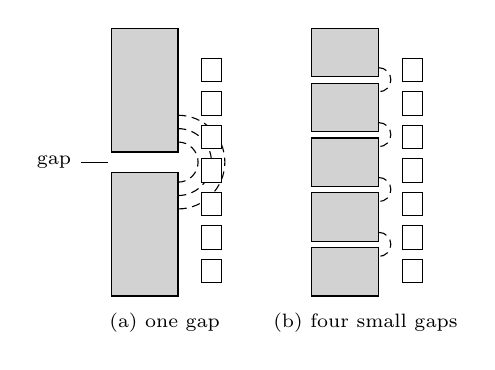
\begin{tikzpicture}[scale=0.85]
					% (a) single gap: centre leg in two parts, fringing field, winding
					\fill[gray!35] (0,1.15) rectangle (1,3);
					\fill[gray!35] (0,-1) rectangle (1,0.85);
					\draw (0,1.15) rectangle (1,3);
					\draw (0,-1) rectangle (1,0.85);
					\foreach \r in {0.3,0.5,0.7}
					\draw[densely dashed] (1,1+\r) arc[start angle=90, end angle=-90, radius=\r];
					\foreach \y in {-0.8,-0.3,0.2,0.7,1.2,1.7,2.2}
					\draw[fill=white] (1.35,\y) rectangle (1.65,\y+0.35);
					\draw (-0.05,1.0) -- (-0.45,1.0) node[left, font=\scriptsize]{gap};
					\node[font=\scriptsize] at (0.8,-1.4) {(a) one gap};
					% (b) quasi-distributed gap
					\begin{scope}[xshift=3.0cm]
						\foreach \y in {-1,-0.18,0.64,1.46,2.28}
						\fill[gray!35] (0,\y) rectangle (1,\y+0.72);
						\foreach \y in {-1,-0.18,0.64,1.46,2.28}
						\draw (0,\y) rectangle (1,\y+0.72);
						\foreach \yc in {-0.23,0.59,1.41,2.23}
						\draw[densely dashed] (1,\yc+0.18) arc[start angle=90, end angle=-90, radius=0.18];
						\foreach \y in {-0.8,-0.3,0.2,0.7,1.2,1.7,2.2}
						\draw[fill=white] (1.35,\y) rectangle (1.65,\y+0.35);
						\node[font=\scriptsize] at (0.8,-1.4) {(b) four small gaps};
					\end{scope}
				\end{tikzpicture}
				\caption{Centre leg (grey), fringing field (dashed) and winding cross-section}
			\end{figure}
		\end{column}
		\begin{column}{0.53\textwidth}
			\small
			\begin{itemize}
				\item The fringing field at a gap enters the nearby conductors and drives eddy currents. The loss grows with the gap length and the frequency.
				\item Keep conductors away from the gap, split it into several small gaps (quasi-distributed gap), or use a distributed-gap material.
				\item Yang et al.: quasi-distributed gaps and a single-layer winding that carries current on both sides. 15\,$\mu$H at 3\,MHz and 2\,A: $Q=720$ with solid copper, 980 with litz wire; 19\,\% lower converter loss at 250\,W.
				\item About twice the $Q$ of a conventional inductor with the same core material (Perreault).
			\end{itemize}
		\end{column}
	\end{columns}
	\blfootnote{Sources: Hu and Sullivan, IEEE IAS 1997; Yang et al., IEEE TPEL, 2019; Perreault, APEC 2024 plenary.}
\end{frame}

%%%%%%%%%%%%%%%%%%%%%%%%%%%%%%%%%%%%%%%%%%%%%%%%%%%%%%%%%%%%%
%% Demo %%
%%%%%%%%%%%%%%%%%%%%%%%%%%%%%%%%%%%%%%%%%%%%%%%%%%%%%%%%%%%%%
\begin{frame}
	\frametitle{Ferrite or air core}
	\begin{columns}[T]
		\begin{column}{0.5\textwidth}
			\textbf{Demonstration}
			\begin{enumerate}
				\item Two inductors of about 1\,$\mu$H: a few turns on a NiZn toroid, and an air-core solenoid.
				\item Impedance analyser from 100\,kHz to 30\,MHz (L5): $|Z|$, phase and $Q$.
				\item A metal plate is brought close to each inductor.
			\end{enumerate}
		\end{column}
		\begin{column}{0.47\textwidth}
			\textbf{Write down}
			\begin{itemize}
				\item the maximum $Q$ and its frequency, and the self-resonance of each inductor
				\item the volume of each inductor
				\item the change of $L$ and $Q$ near the plate
			\end{itemize}
			\begin{block}{Key message}
				A core keeps the inductor small and its field contained up to the low MHz range. At higher frequency, or for very high $Q$, an air core often wins, at the cost of size and stray field.
			\end{block}
		\end{column}
	\end{columns}
\end{frame}

%%%%%%%%%%%%%%%%%%%%%%%%%%%%%%%%%%%%%%%%%%%%%%%%%%%%%%%%%%%%%
%% Material map %%
%%%%%%%%%%%%%%%%%%%%%%%%%%%%%%%%%%%%%%%%%%%%%%%%%%%%%%%%%%%%%
\subsection{Choosing a material}

\begin{frame}
	\frametitle{Material selection map}
	\begin{columns}[T]
		\begin{column}{0.6\textwidth}
			\begin{figure}
				\centering
				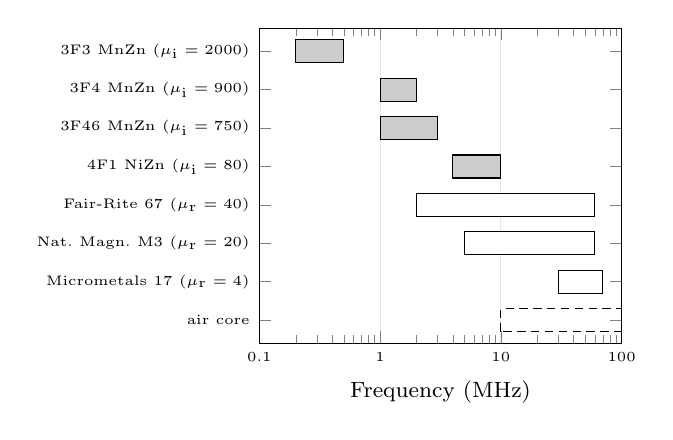
\begin{tikzpicture}
					\begin{axis}[
							xmode=log, scale only axis, width=4.6cm, height=4.0cm,
							xmin=0.1, xmax=100, ymin=0.4, ymax=8.6,
							xtick={0.1,1,10,100}, xticklabels={0.1,1,10,100},
							ytick={1,2,3,4,5,6,7,8},
							yticklabels={air core, Micrometals 17 ($\mu_\mathrm{r}=4$), Nat.\ Magn.\ M3 ($\mu_\mathrm{r}=20$), Fair-Rite 67 ($\mu_\mathrm{r}=40$), 4F1 NiZn ($\mu_\mathrm{i}=80$), 3F46 MnZn ($\mu_\mathrm{i}=750$), 3F4 MnZn ($\mu_\mathrm{i}=900$), 3F3 MnZn ($\mu_\mathrm{i}=2000$)},
							xlabel={Frequency (MHz)},
							xmajorgrids, grid style={gray!20},
							tick label style={font=\tiny}, label style={font=\footnotesize},
						]
						\draw[fill=gray!40] (axis cs:0.2,7.7) rectangle (axis cs:0.5,8.3);
						\draw[fill=gray!40] (axis cs:1,6.7) rectangle (axis cs:2,7.3);
						\draw[fill=gray!40] (axis cs:1,5.7) rectangle (axis cs:3,6.3);
						\draw[fill=gray!40] (axis cs:4,4.7) rectangle (axis cs:10,5.3);
						\draw[fill=white] (axis cs:2,3.7) rectangle (axis cs:60,4.3);
						\draw[fill=white] (axis cs:5,2.7) rectangle (axis cs:60,3.3);
						\draw[fill=white] (axis cs:30,1.7) rectangle (axis cs:70,2.3);
						\draw[densely dashed] (axis cs:10,0.7) rectangle (axis cs:100,1.3);
					\end{axis}
				\end{tikzpicture}
				\caption{Grey: frequency range recommended by the manufacturer. White: range of published loss data. Dashed: air core}
			\end{figure}
		\end{column}
		\begin{column}{0.37\textwidth}
			\small
			\begin{itemize}
				\item Up to about 3\,MHz: MnZn power ferrites, the newest grades at the top of this range.
				\item 3--30\,MHz: NiZn and low-permeability ferrites with $\mu_\mathrm{r}=20$--80.
				\item Above about 30\,MHz: $\mu_\mathrm{r}\leq20$, powders or air core.
				\item Check the data at your frequency, flux density, temperature and waveform.
			\end{itemize}
		\end{column}
	\end{columns}
	\blfootnote{Sources: Ferroxcube data sheets; Hanson et al., 2016; Han et al., 2012; Perreault, APEC 2024.}
\end{frame}

%%%%%%%%%%%%%%%%%%%%%%%%%%%%%%%%%%%%%%%%%%%%%%%%%%%%%%%%%%%%%
%% Magnetics in the briefs %%
%%%%%%%%%%%%%%%%%%%%%%%%%%%%%%%%%%%%%%%%%%%%%%%%%%%%%%%%%%%%%
\begin{frame}
	\frametitle{Magnetics in the briefs}
	\begin{table}
		\centering
		\footnotesize
		\begin{tabular}{|l|>{\raggedright\arraybackslash}p{3.0cm}|>{\raggedright\arraybackslash}p{9.6cm}|}
			\hline
			   & \textbf{Brief}           & \textbf{Magnetic component and core-loss question}                                                                    \\
			\hline
			B1 & ZVS GaN buck, 1--3\,MHz  & inductor with triangular flux and large ripple; iGSE with the actual duty cycle; DC bias; fringing at the gap      \\
			B2 & LLC DCX, 1\,MHz          & planar transformer, nearly symmetric flux; $P_\mathrm{fe}=(2/\beta)P_\mathrm{cu}$ with integer turns                 \\
			B3 & DAB, 0.5--1\,MHz         & transformer and series inductor; triangular flux, or trapezoidal with zero-voltage intervals under extended phase shift: iGSE and relaxation               \\
			B4 & 6.78\,MHz class E        & matching inductors and coil $Q$: NiZn (e.g.\ 67) or air core                                                       \\
			B5 & 13.56\,MHz VHF           & resonant inductors: air core or $\mu_\mathrm{r}\leq40$; $Q$ and self-resonance                                      \\
			B6 & hybrid SC, 48\,V         & small resonant inductors with DC current: bias and loss at $\leq1$\,MHz                                            \\
			\hline
		\end{tabular}
		\caption{Milestone M1 (25.11.): devices and magnetics pre-design with material, $\hat{B}$, core and winding loss}
	\end{table}
\end{frame}

%%%%%%%%%%%%%%%%%%%%%%%%%%%%%%%%%%%%%%%%%%%%%%%%%%%%%%%%%%%%%
%% Key messages %%
%%%%%%%%%%%%%%%%%%%%%%%%%%%%%%%%%%%%%%%%%%%%%%%%%%%%%%%%%%%%%
\begin{frame}
	\frametitle{Key messages}
	\begin{enumerate}
		\item Above a few tens of kHz core loss, not saturation, limits $\hat{B}$: at constant loss density $f\hat{B}\propto f^{1-\alpha/\beta}$.
		\item The performance factor shows where a material is best. With single-layer windings the gain of frequency is $\hat{B}f^{3/4}$: about $\times1.4$ from 2 to 10\,MHz.
		\item Minimum total loss at $P_\mathrm{fe}=(2/\beta)P_\mathrm{cu}$, not at equal losses. The minimum is flat.
		\item Above about 3\,MHz NiZn and low-permeability ferrites; $\mu_\mathrm{r}=20$--40 is enough, the gap does the rest.
		\item Steinmetz holds for sinusoids. The iGSE handles PWM flux; relaxation and DC bias need measured data.
		\item Small magnetics are limited by efficiency: few, large components.
	\end{enumerate}
\end{frame}

%%%%%%%%%%%%%%%%%%%%%%%%%%%%%%%%%%%%%%%%%%%%%%%%%%%%%%%%%%%%%
%% Exit ticket %%
%%%%%%%%%%%%%%%%%%%%%%%%%%%%%%%%%%%%%%%%%%%%%%%%%%%%%%%%%%%%%
% Two pages: questions (page 1) and answers (page 2).
\begin{frame}<handout:1-2>
	\frametitle{Exit questions}
	\begin{varblock}[\textwidth]{Three questions, one minute each}
		\begin{enumerate}
			\item A material has $\alpha=1.6$ and $\beta=2.4$. By how much does the VA of a given core change when the frequency is doubled at constant loss density?
			\item A transformer designed for minimum loss has 1.8\,W total loss and $\beta=2.5$. How large are core and winding loss?
			\item Why is the data-sheet loss at the same $\hat{B}$ too optimistic for a buck inductor with $D=0.1$?
		\end{enumerate}
	\end{varblock}
	\onslide<2-|handout:2>{
		\begin{enumerate}
			\item $f\hat{B}\propto f^{1-\alpha/\beta}=f^{1/3}$: $2^{1/3}=1.26$, i.e.\ 26\,\% more.
			\item $P_\mathrm{fe}=0.8\,P_\mathrm{cu}$: $P_\mathrm{cu}=1.0$\,W, $P_\mathrm{fe}=0.8$\,W.
			\item The flux rises in 10\,\% of the period; the loss follows $|\mathrm{d}B/\mathrm{d}t|^{\alpha}$: about 36\,\% more for $\alpha=1.5$ (iGSE). The DC bias of the inductor raises the loss further.
		\end{enumerate}
	}
\end{frame}

%%%%%%%%%%%%%%%%%%%%%%%%%%%%%%%%%%%%%%%%%%%%%%%%%%%%%%%%%%%%%
%% References %%
%%%%%%%%%%%%%%%%%%%%%%%%%%%%%%%%%%%%%%%%%%%%%%%%%%%%%%%%%%%%%
\begin{frame}
	\frametitle{References}
	\scriptsize
	\begin{itemize}
		\item A.\,J. Hanson, J.\,A. Belk, S. Lim, C.\,R. Sullivan, D.\,J. Perreault, ``Measurements and performance factor comparisons of magnetic materials at high frequency,'' IEEE Trans.\ Power Electron., vol.\ 31, no.\ 11, pp.\ 7909--7925, 2016.
		\item C.\,R. Sullivan, B.\,A. Reese, A.\,L.\,F. Stein, P.\,A. Kyaw, ``On size and magnetics: Why small efficient power inductors are rare,'' 3D-PEIM 2016.
		\item D.\,J. Perreault, ``Opportunities, progress and challenges in high-frequency power conversion,'' plenary, IEEE APEC 2024.
		\item R.\,W. Erickson, D. Maksimovi\'c, \textit{Fundamentals of Power Electronics}, 3rd ed., Springer, 2020, Ch.\ 10--12.
		\item K. Venkatachalam, C.\,R. Sullivan, T. Abdallah, H. Tacca, ``Accurate prediction of ferrite core loss with nonsinusoidal waveforms using only Steinmetz parameters,'' IEEE COMPEL 2002, pp.\ 36--41.
		\item J. M\"uhlethaler, J. Biela, J.\,W. Kolar, A. Ecklebe, ``Improved core-loss calculation for magnetic components employed in power electronic systems,'' IEEE Trans.\ Power Electron., vol.\ 27, no.\ 2, pp.\ 964--973, 2012.
		\item H. Li et al., ``How MagNet: Machine learning framework for modeling power magnetic material characteristics,'' IEEE Trans.\ Power Electron., vol.\ 38, no.\ 12, pp.\ 15829--15853, 2023; M. Chen et al., ``MagNet Challenge for data-driven power magnetics modeling,'' IEEE Open J.\ Power Electron., vol.\ 6, pp.\ 883--898, 2025.
		\item R.\,S. Yang, A.\,J. Hanson, B.\,A. Reese, C.\,R. Sullivan, D.\,J. Perreault, ``A low-loss inductor structure and design guidelines for high-frequency applications,'' IEEE Trans.\ Power Electron., vol.\ 34, no.\ 10, pp.\ 9993--10005, 2019.
	\end{itemize}
\end{frame}

\begin{frame}
	\frametitle{References (cont.)}
	\scriptsize
	\begin{itemize}
		\item J. Hu, C.\,R. Sullivan, ``The quasi-distributed gap technique for planar inductors: design guidelines,'' IEEE IAS Annual Meeting, 1997.
		\item J.\,L. Snoek, ``Dispersion and absorption in magnetic ferrites at frequencies above one Mc/s,'' Physica, vol.\ 14, no.\ 4, pp.\ 207--217, 1948.
		\item C. Beatrice et al., ``The temperature dependence of magnetic losses in CoO-doped Mn-Zn ferrites,'' J.\ Appl.\ Phys., vol.\ 126, 143902, 2019.
		\item C. \'O Math\'una, N. Wang, S. Kulkarni, S. Roy, ``Review of integrated magnetics for power supply on chip (PwrSoC),'' IEEE Trans.\ Power Electron., vol.\ 27, no.\ 11, pp.\ 4799--4816, 2012.
		\item Data sheets: Ferroxcube 3F3, 3F4, 3F46, 4F1; Fair-Rite 67.
	\end{itemize}
\end{frame}
